\documentclass[12pt]{article}

\usepackage{graphicx}
\usepackage[font=footnotesize]{subfig}
\usepackage{float}
\usepackage{xepersian}
\settextfont[Scale=1]{XB Niloofar}
\setlatintextfont[Scale=0.9]{Times New Roman}
\title{پروژه پایانی درس یادگیری عمیق}
\author{کورش تقی‌پور پاسدار}
\begin{document}
	\maketitle
	\newpage
	\tableofcontents
	\newpage
	\section{\lr{Preprocess}}
	در این بخش، به \lr{import} کردن کتابخانه‌های لازم و همچنین دانلود دیتاست \lr{Flickr8k} و \lr{import} کردن ترجمه‌ای که قبلا انجام داده‌ایم می‌پردازیم.
	\subsection{\lr{Import Libraries}}
	\begin{figure}[H]
		\centering
		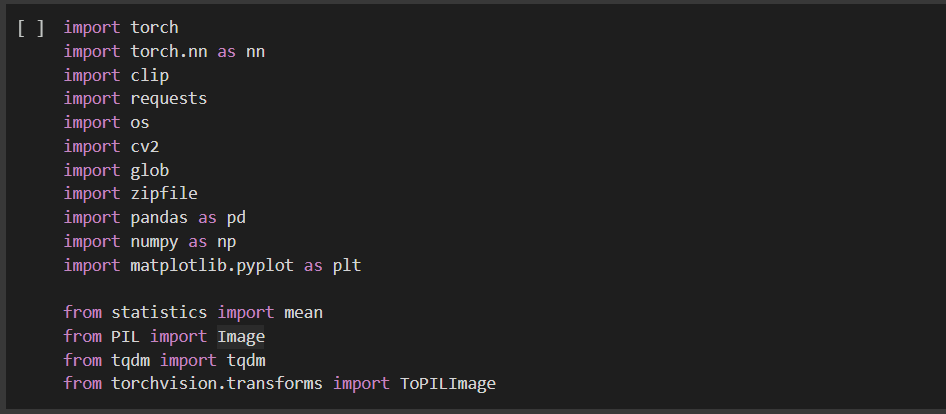
\includegraphics[width=0.9\linewidth]{pic_1}
	\end{figure}
	\subsection{\lr{Preprocess Flickr8k Dataset}}
	\subsubsection{\lr{Download and Unzip Dataset}}
	در ابتدا تابعی برای دانلود و ذخیره دیتاست تعریف می‌کنیم.
	\begin{figure}[H]
		\centering
		\subfloat{
		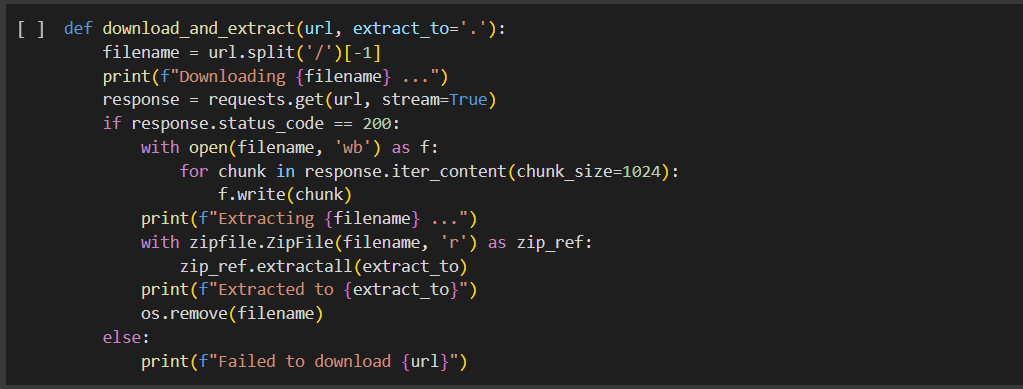
\includegraphics[width=0.4\linewidth]{pic_2}}
		\quad \quad
		\subfloat{
		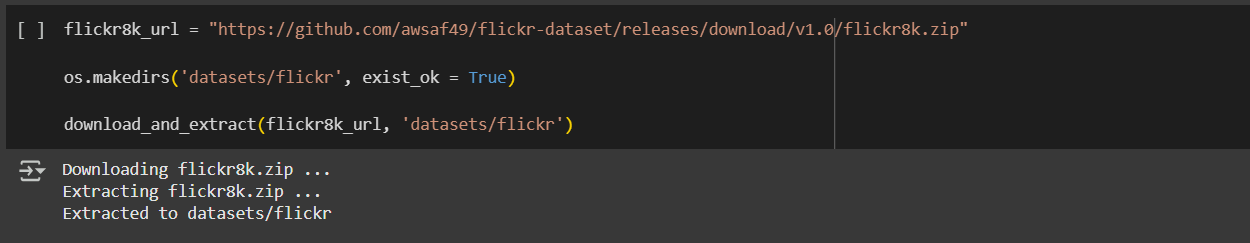
\includegraphics[width=0.4\linewidth]{pic_3}
		}
	\end{figure}
	\subsubsection{\lr{Read and Save Captions}}
	سپس به خواندن و استخراج کپشن‌ها از این دیتاست می‌پردازیم.
	\begin{figure}[H]
		\centering
		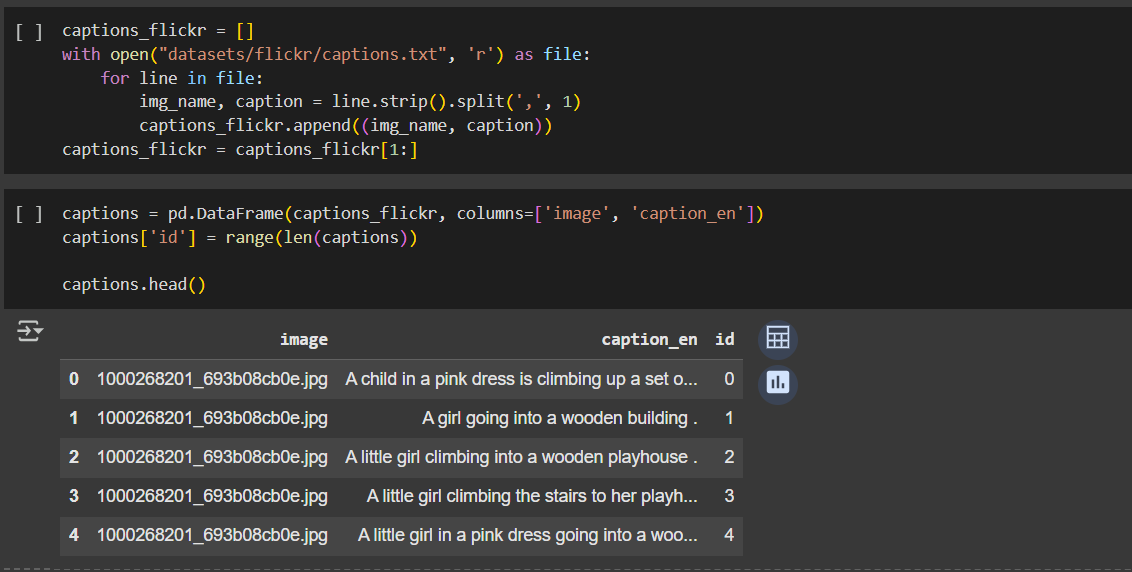
\includegraphics[width=0.9\linewidth]{pic_4}
	\end{figure}
	\subsubsection{\lr{Extract Translated Captions and Merge}}
	سپس کپشن‌های فارسی ترجمه شده از قبل را از فایل‌ها خوانده و با کپشن‌های انگلیسی در یک دیتافریم \LTRfootnote{\lr{DataFrame}} قرار می‌دهیم.
	\begin{figure}[H]
		\centering
		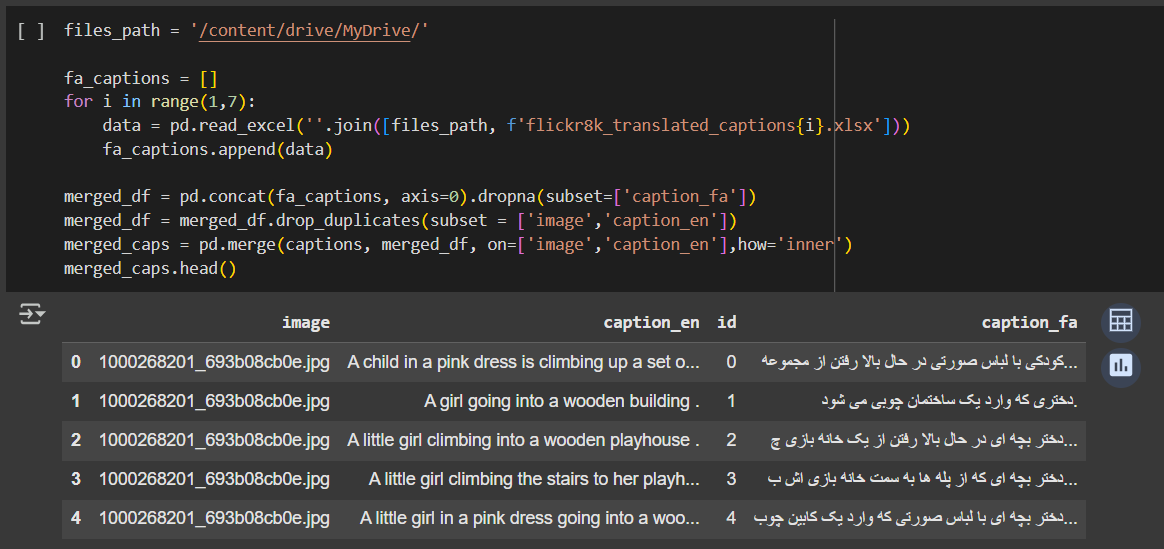
\includegraphics[width=0.9\linewidth]{pic_5}
	\end{figure}
	\subsubsection{\lr{Check Translation Validity}}
	سپس با استفاده از یک مدل هوش مصنوعی \lr{Sentence Transformer} به مقایسه و بررسی کبفیت ترجمه می‌پردازیم.
	\begin{figure}[H]
		\centering
		\subfloat[
		بررسی کیفیت ترجمه داده‌ها و نمایش میانگین تطابق
		]{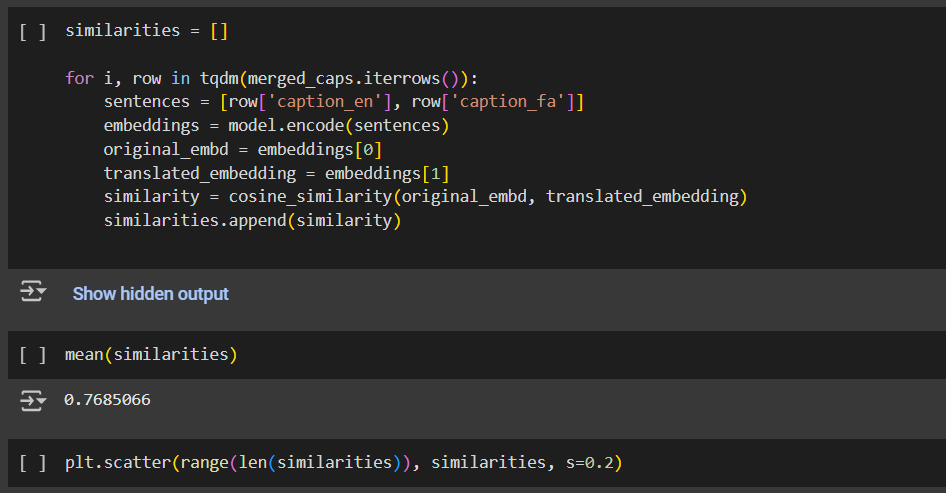
\includegraphics[width=0.4\linewidth]{pic_6}}
		\quad \quad
		\subfloat[
		رسم بصری هر یک از مقادیر تطابق
		]{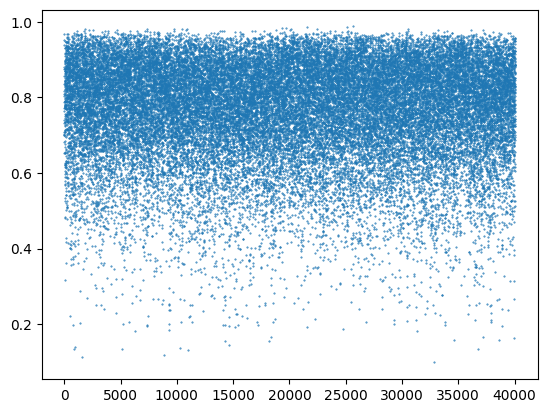
\includegraphics[width=0.4\linewidth]{pic_7}}
	\end{figure}
	\section{\lr{Define Model}}
	حال در اینجا به تعریف مدل می‌پردازیم. برای این کار، از مدل \lr{CLIP} استفاده کرده‌ایم و به تعریف دقیق‌تر، یک مدل \lr{pretrain} شده را استفاده می‌کنیم که سعی می‌کنیم با \lr{Fine-tune} کردن آن، برای تسک مورد نظر آموزش دهیم.
	\begin{figure}[H]
		\centering
		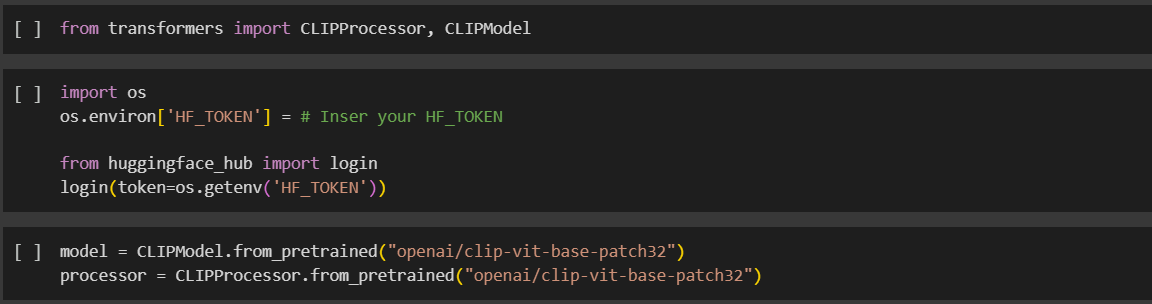
\includegraphics[width=0.9\linewidth]{pic_8}
	\end{figure}
	\section{\lr{Define Dataset}}
	در اینجا، دیتاست خود را تعریف می‌کنیم. منظور از تعریف دیتاست، تعریف \textbf{کلاس} \LTRfootnote{\lr{Class}} دیتاست است تا داده‌ها را از آن بگیریم.
	\begin{figure}[H]
		\centering
		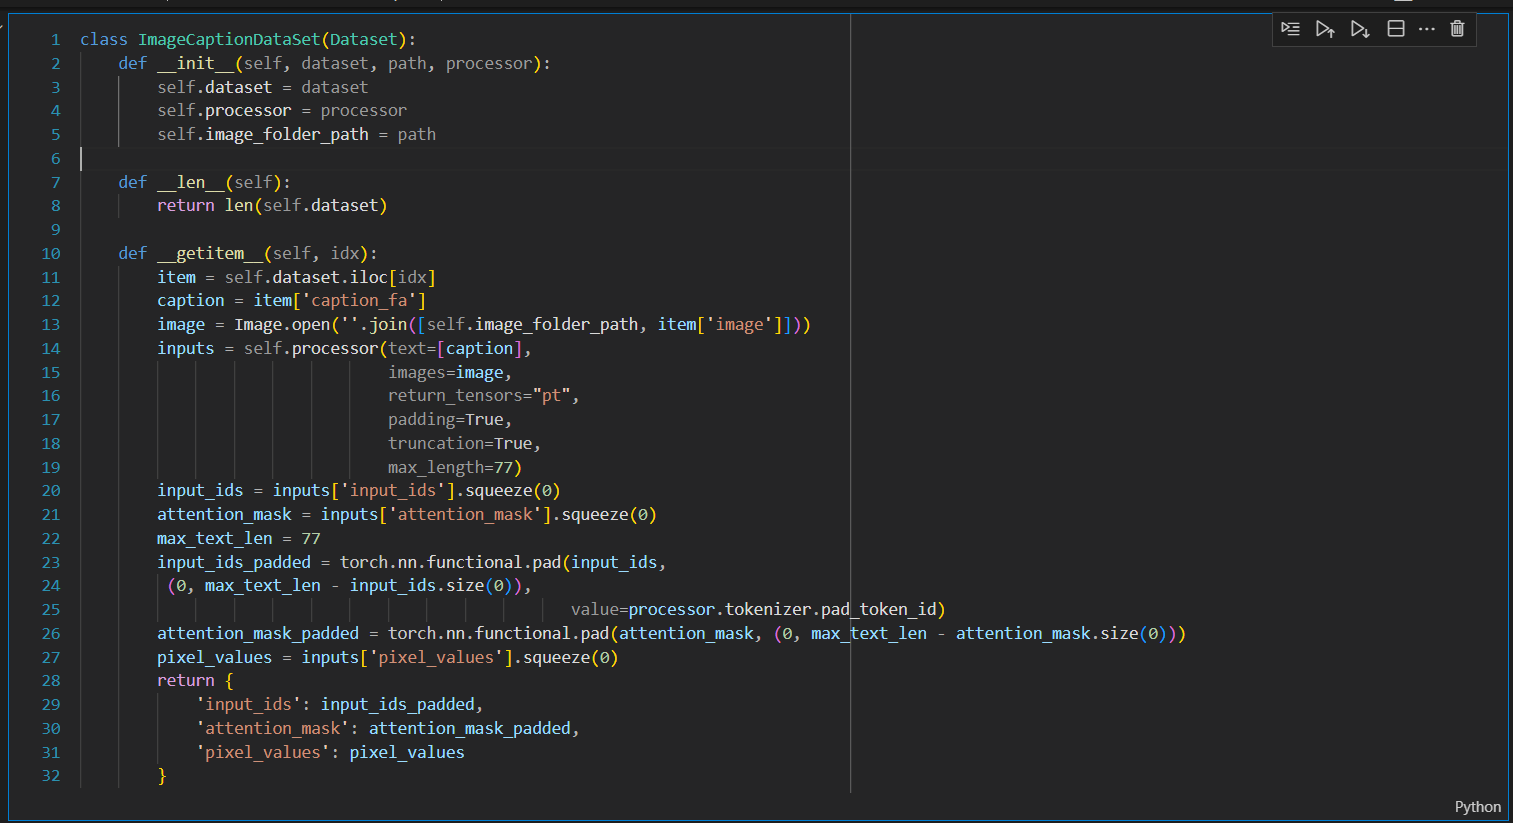
\includegraphics[width=0.9\linewidth]{pic_9}
	\end{figure}
	سپس داده‌های آموزشی و تست را با استفاده از \lr{train test split} از کتابخانه \lr{sklearn} جدا می‌کنیم.
	\begin{figure}[H]
		\centering
		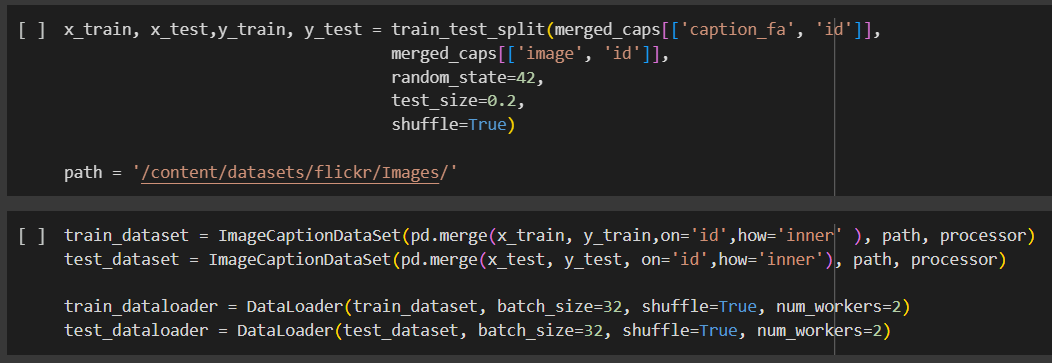
\includegraphics[width=0.9\linewidth]{pic_10}
	\end{figure}
	\section{\lr{Fine-Tune}}
	حال به بخش \lr{Fine-Tune} مدل می‌رسیم.
	\subsection{\lr{Freeze Some Layers}}
	با توجه به اینکه این یک شبکه‌ی از پیش آموزش دیده است، پس توانایی برقراری ارتباط بین تصویر و متن را دارد. لازم است که بخش‌های استخراج ویژگی از تصویر و همچنین برقراری ارتباط بین ویژگی‌های تصویر و متن ثابت مانده و تنها استخراج ویژگی از متن تغییر کند. به همین دلیل، به فریز کردن بخش بزرگی از شبکه می‌پردازیم.
	\begin{figure}[H]
		\centering
		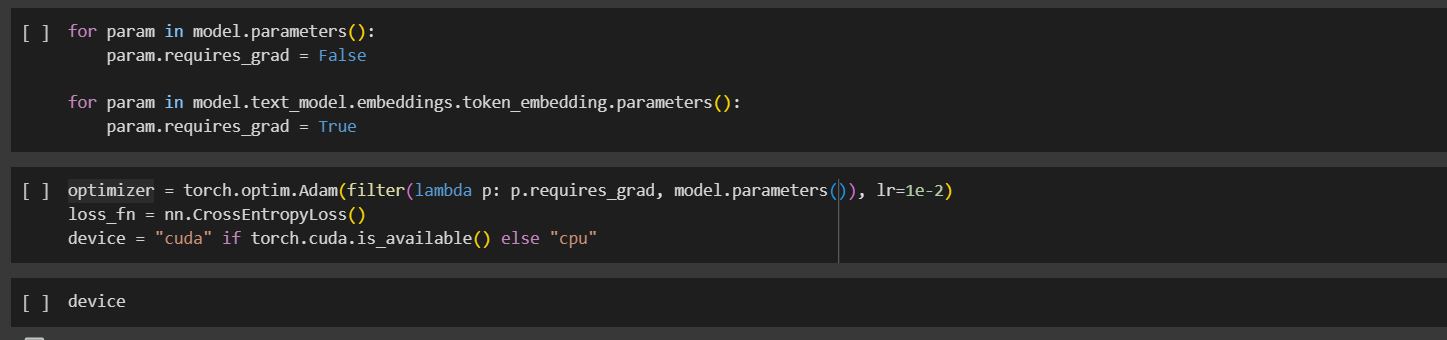
\includegraphics[width=0.9\linewidth]{pic_11}
	\end{figure}
	همچنین از بهینه‌ساز \lr{Adam} و تابع \lr{CrossEntropyLoss} برای محاسبه خطا استفاده می‌کنیم.
	
	سپس به تعریف تابع \lr{train} می‌پردازیم.
	\begin{figure}[H]
		\centering
		\subfloat{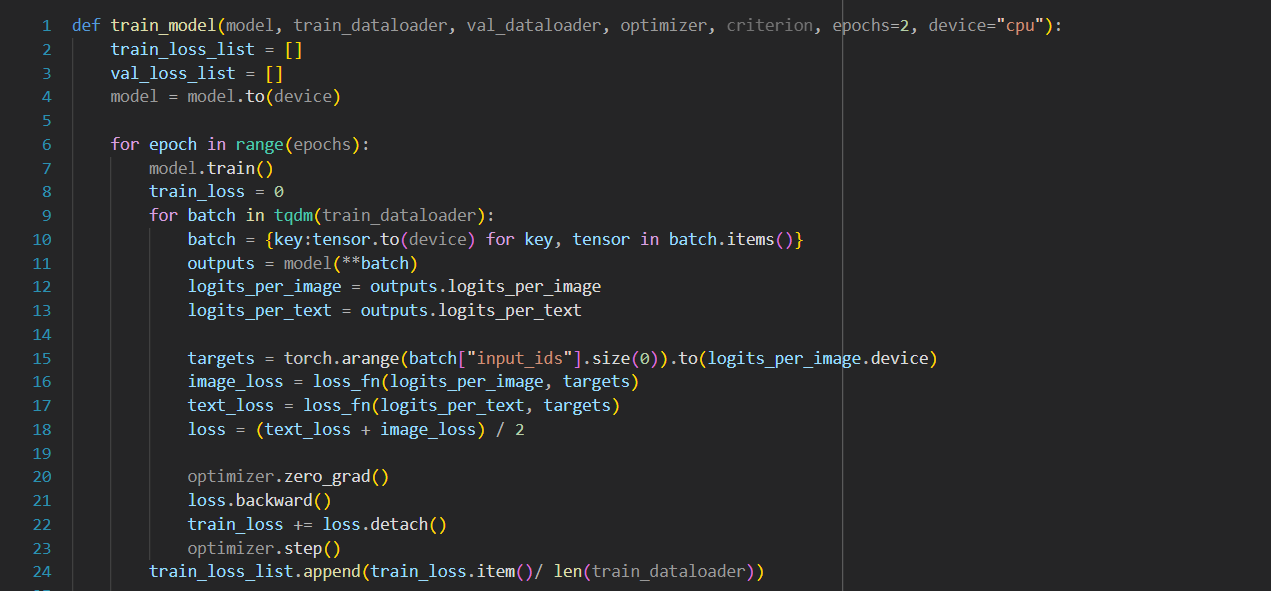
\includegraphics[width=0.4\linewidth]{pic_12}}
		\quad \quad
		\subfloat{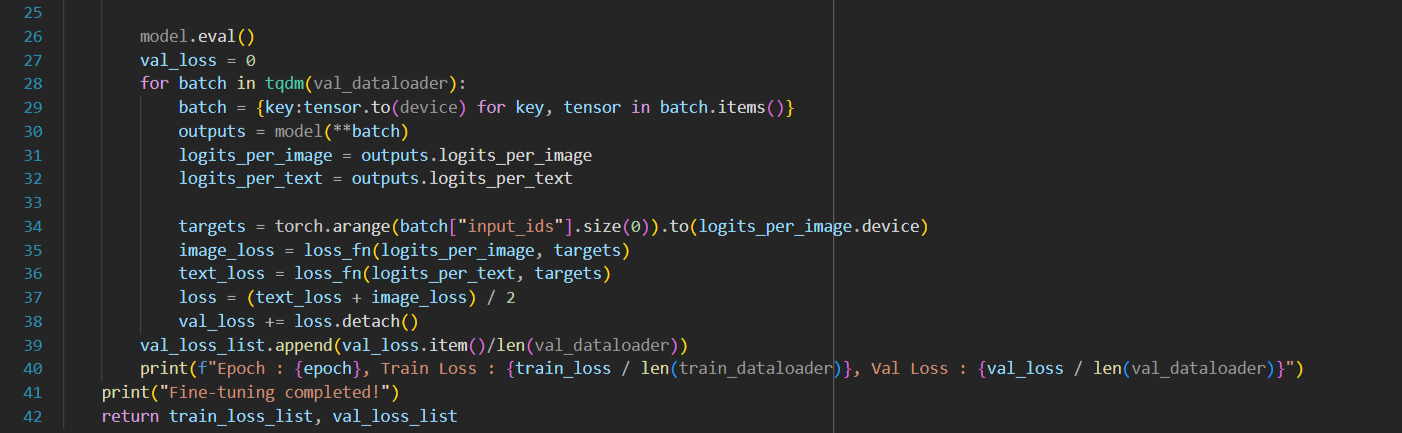
\includegraphics[width=0.4\linewidth]{pic_13}}
	\end{figure}
	سپس به آموزش مدل می‌پردازیم.
	\begin{figure}[H]
		\centering
		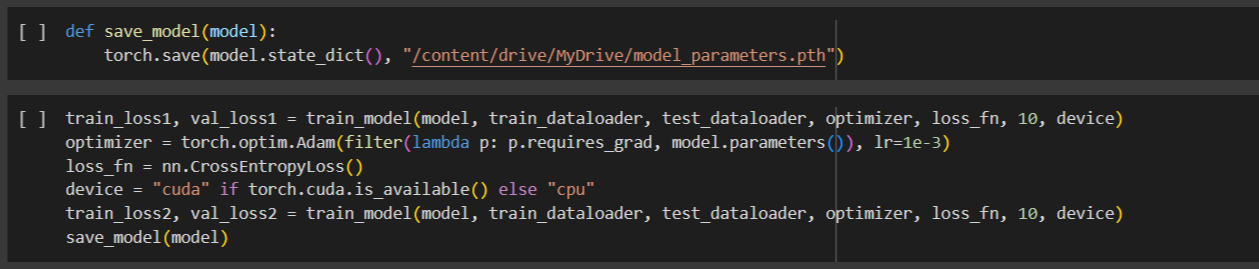
\includegraphics[width=0.9\linewidth]{pic_14}
	\end{figure}
	\section{\lr{Import Evaluation Data}}
	حال در اینجا به ویدیو‌های تست، استخراج فریم‌ها و \lr{encode} کردن آنها به آرایه‌های تنسور \LTRfootnote{\lr{Tensor Array}} می‌پردازیم.
	\begin{figure}[H]
		\centering
		\subfloat[
		تابع استخراج فریم‌های یک ویدیو
		]{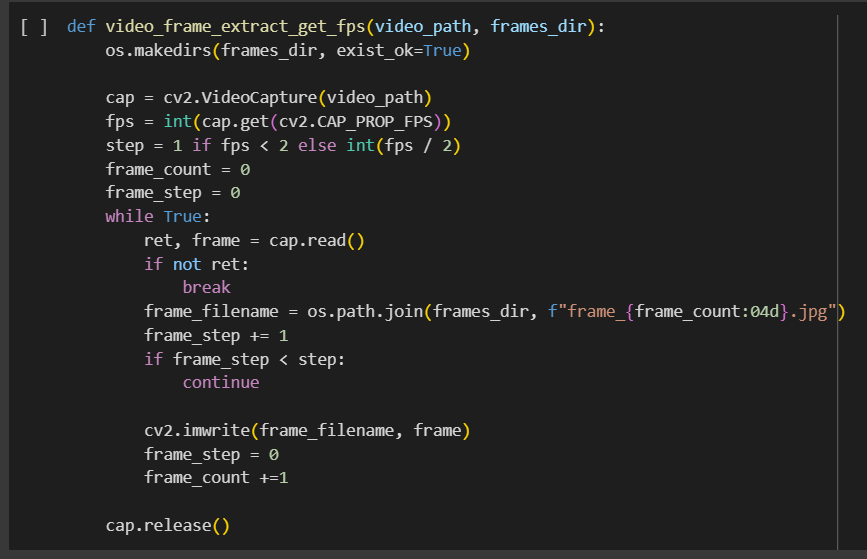
\includegraphics[width=0.4\linewidth]{pic_15}}
		\quad \quad
		\subfloat[
		تابعی برای استخراج فریم‌های تمام ویدیو‌های داخل یک پوشه
		]{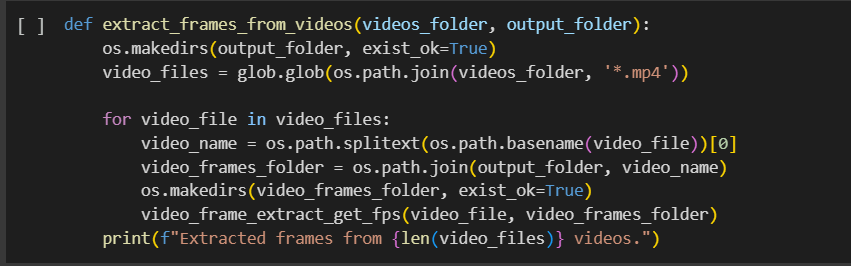
\includegraphics[width=0.4\linewidth]{pic_16}}
		\quad \quad
		\subfloat[
		تابعی برای \lr{encode} کردن ویدیو‌ها و تبدیل آنها به یک \lr{Tensor}
		]{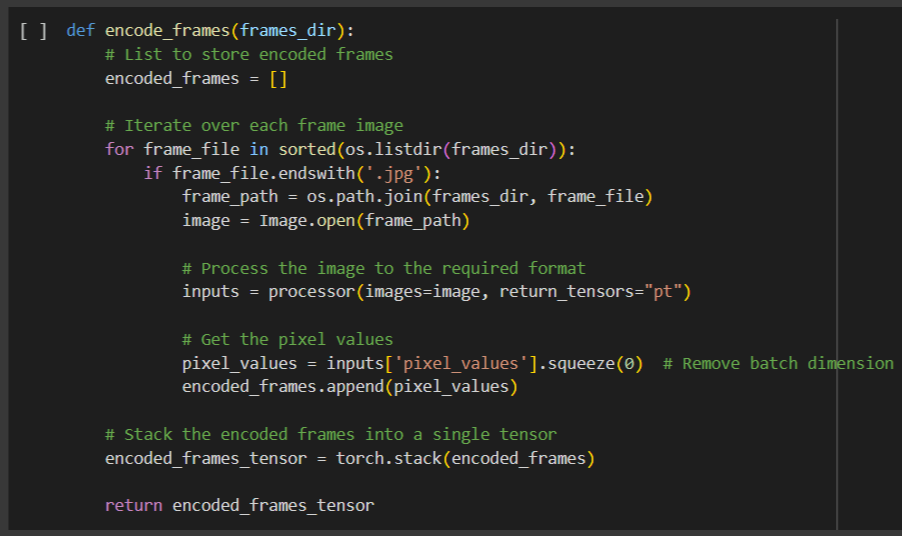
\includegraphics[width=0.4\linewidth]{pic_17}}
		\quad \quad
		\subfloat[
		تابعی برای استخراج \lr{tensor} های تمام ویدیو‌ها. این تابع دربردارنده تابع‌های قبلی است.
		]{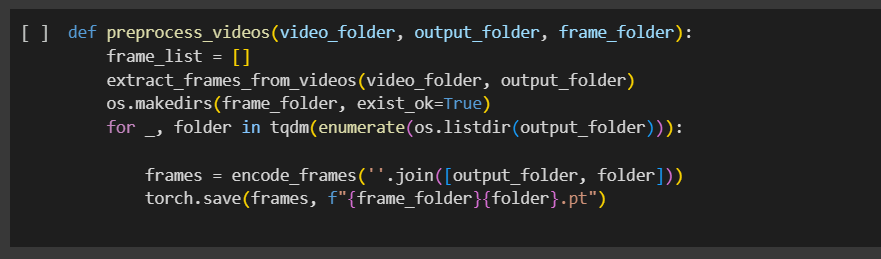
\includegraphics[width=0.4\linewidth]{pic_18}}
		\quad \quad
		\subfloat[
		تابعی بری لود کردن \lr{tensor} ها
		]{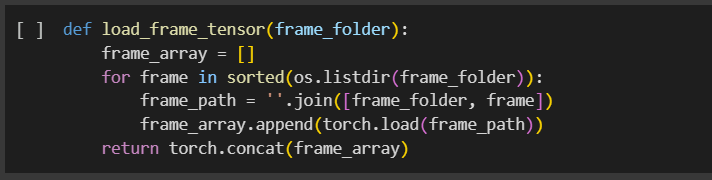
\includegraphics[width=0.4\linewidth]{pic_19}}
	\end{figure}
	\section{\lr{Text-to-Image Retrieval}}
	حال به تابع یافتن فریم ویدیو براساس متن ورودی می‌پردازیم. در این تابع براساس متن ورودی و آرایه‌ای که در قبل از ویدیو‌ها ساختیم، بهترین \lr{k} فریم را پیدا می‌کنیم.  این مقدار قابل تغییر است.
	\begin{figure}[H]
		\centering
		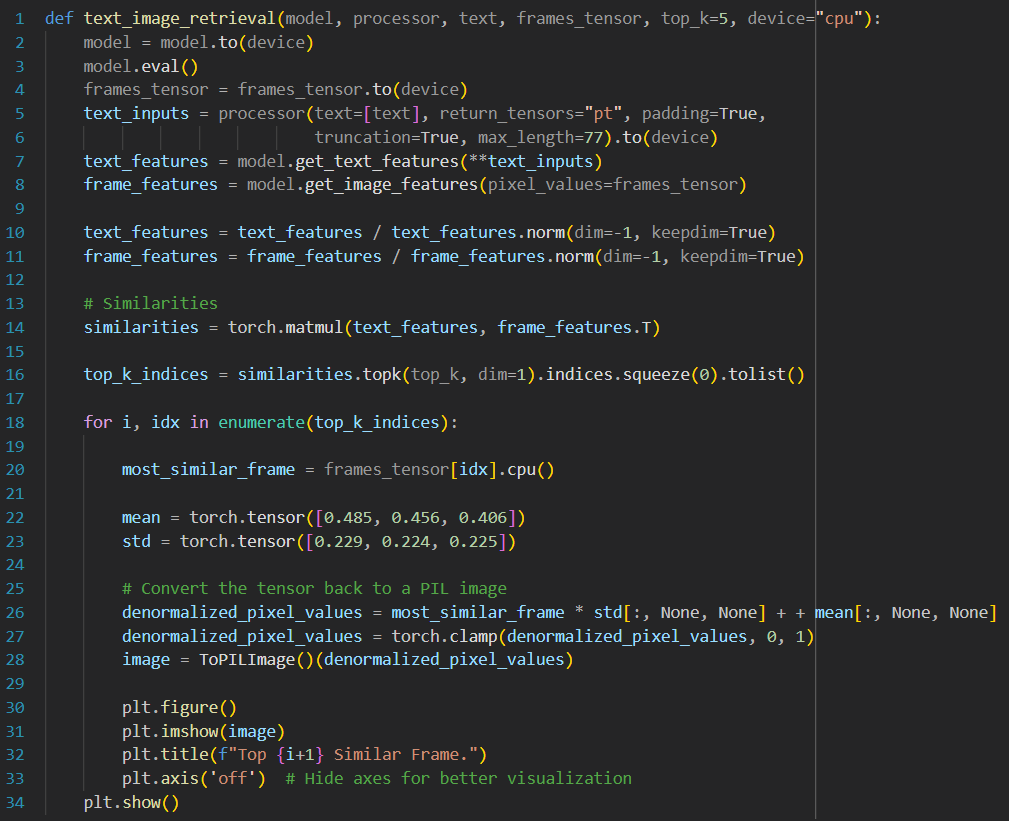
\includegraphics[width=0.9\linewidth]{pic_20}
	\end{figure} 
\end{document}